\section{ЗАДАНИЕ}

Используя хвостовую рекурсию, разработать, комментируя аргументы, эффективную программу, позволяющую:

\begin{enumerate}
    \item Сформировать список из элементов числового списка, больших заданного значения;
    \item Сформировать список из элементов, стоящих на нечетных позициях исходного списка (нумерация от 0);
    \item Удалить заданный элемент из списка (один или все вхождения);
    \item Преобразовать список в множество (можно использовать ранее разработанные процедуры).
\end{enumerate}

\begin{lstlisting}[caption=Текст программы]
domains
	list = integer*.
	index = integer.

predicates
	moreThat(list, integer, list).
	listOdd(list, list).
	listOdd(list, list, index).
	removeFirst(list, integer, list).
	removeAll(list, integer, list).
	set(list, list).

clauses
	moreThat([], _, []) :- !.
	moreThat([Head|Tail], Number, Result) :-
		Head > Number,
		moreThat(Tail, Number, TailResult),
		Result = [Head|TailResult].
	moreThat([Head|Tail], Number, Result) :-
		Head <= Number,
		moreThat(Tail, Number, Result).

	listOdd(List, Result) :- listOdd(List, Result, 0).
	listOdd([], [], _) :- !.
	listOdd([_|Tail], Result, Index) :-
		Index mod 2 = 0,
		NextIndex = Index + 1,
		listOdd(Tail, Result, NextIndex).
	listOdd([Head|Tail], Result, Index) :-
		Index mod 2 = 1,
		NextIndex = Index + 1,
		listOdd(Tail, TailResult, NextIndex),
		Result = [Head|TailResult].

	removeFirst([], _, []) :- !.
	removeFirst([Head|Tail], Number, Result) :-
		Head = Number,
		Result = Tail, !.
	removeFirst([Head|Tail], Number, Result) :-
		Head <> Number,
		removeFirst(Tail, Number, TailResult),
		Result = [Head|TailResult].

	removeAll([], _, []) :- !.
	removeAll([Head|Tail], Number, Result) :-
		Head = Number,
		removeAll(Tail, Number, Result).
	removeAll([Head|Tail], Number, Result) :-
		Head <> Number,
		removeAll(Tail, Number, TailResult),
		Result = [Head|TailResult].

	set([], []) :- !.
	set([Head|Tail], Set) :-
		removeAll(Tail, Head, NextTail),
		set(NextTail, TailSet),
		Set = [Head|TailSet].

goal
	moreThat([4, 7, 1, 2, 8], 5, ResultMore);
	listOdd([1, 2, 3, 4, 5], ResultOdd);
	removeFirst([1, 2, 3, 2, 4], 2, ResultFirst);
	removeAll([1, 2, 3, 2, 4], 2, ResultAll);
	set([1, 2, 3, 4, 1, 2, 5, 2, 1, 2, 6, 8, 2, 6, 8], Set).
\end{lstlisting}

\section{РЕЗУЛЬТАТ РАБОТЫ}

\begin{figure}[H]
    \centering
    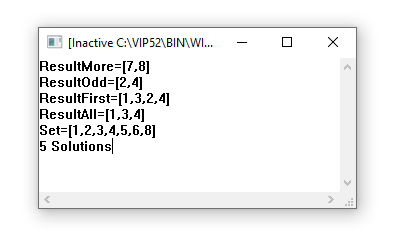
\includegraphics{img/result.png}
    \caption{Результат работы программы}
\end{figure}
